\appendix

\section{Appendix: example of usage and related output}
In this appendix we want to offer some insights of how DALILA code works and the possible outcomes we can obtain. All the experiments are performed on the ORL database of faces \footnote{The database is available for download at the link \url{http://www.cl.cam.ac.uk/research/dtg/attarchive/facedatabase.html}}. This database is saved as a matrix within the library with 400 samples and $112\times 92$ features.

In order to perform Dictionary Learning on this dataset we firstly need to flatten the matrices into arrays and then apply the fitting procedure. In this estimator we are using an arbitrary number of atoms that we choose randomly and we impose non-negativity on both the matrices since we are dealing with gray scale images that have values in the range of [0,255]. 
\begin{lstlisting}[language=Python]
import numpy as np

from dalila.dictionary_learning import DictionaryLearning
from dalila.penalty import L1Penalty

dataset = np.load("/path/to/dalila/folder/dalila/databases/ORL_database.npy")
d1, d2, n = dataset.shape
data = np.empty((n, d1*d2))
for i in range(n):
	data[i,:] = np.ravel(dataset[:,:,i])

estimator = DictionaryLearning(k=60, non_negativity="both")
estimator.fit(data, n_iter=1000)
C, D = estimator.decomposition()
\end{lstlisting}
Some of the results obtained with this code are depicted in Figure \ref{atoms}. Here the most used atoms in the reconstructions are showed.  In Figure \ref{reconstructions}, instead, we show some reconstructions and their original signals to perform a qualitative comparison.
\begin{figure}[H]
\centering
\begin{tabular}{ccccc}
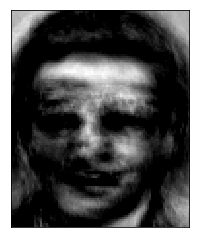
\includegraphics[scale=0.3]{atom_0.png} &
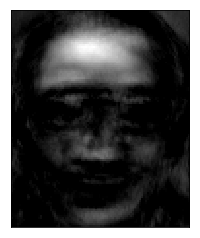
\includegraphics[scale=0.3]{atom_1.png} &
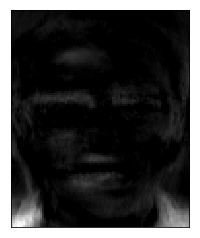
\includegraphics[scale=0.3]{atom_2.png} &
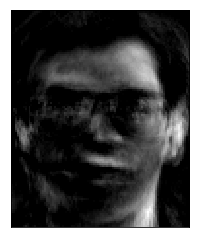
\includegraphics[scale=0.3]{atom_3.png} &
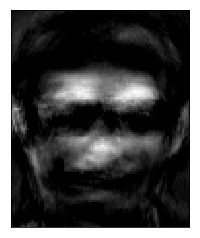
\includegraphics[scale=0.3]{atom_4.png} \\
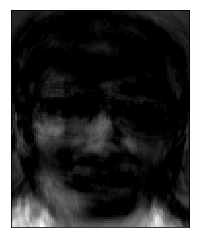
\includegraphics[scale=0.3]{atom_5.png} &
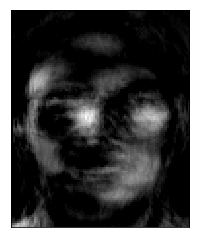
\includegraphics[scale=0.3]{atom_6.png} &
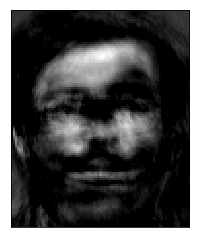
\includegraphics[scale=0.3]{atom_7.png} &
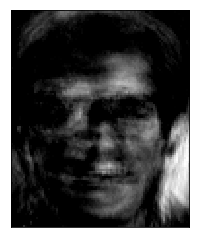
\includegraphics[scale=0.3]{atom_8.png} &
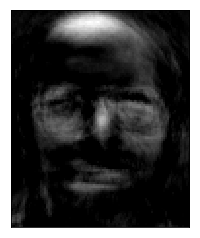
\includegraphics[scale=0.3]{atom_9.png} \\
\end{tabular}
\caption{The ten more recurrent atoms for the reconstruction of the samples in ORL dataset.}
\label{atoms}
\end{figure}

\begin{figure}[H]
\centering
\begin{tabular}{ccc}
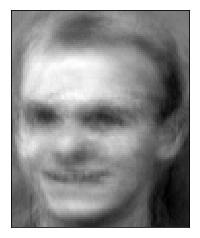
\includegraphics[scale=0.5]{reconstruction1.png} &
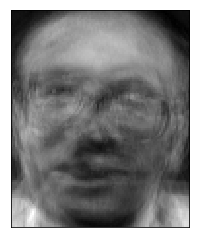
\includegraphics[scale=0.5]{reconstruction2.png} &
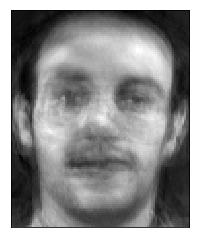
\includegraphics[scale=0.5]{reconstruction3.png}\\
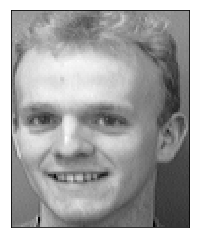
\includegraphics[scale=0.5]{original1.png} &
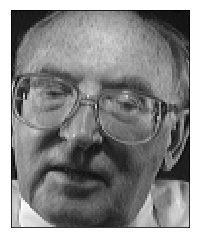
\includegraphics[scale=0.5]{original2.png} &
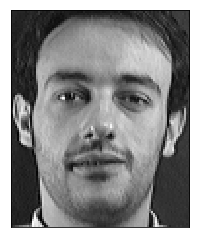
\includegraphics[scale=0.5]{original3.png}\\
\end{tabular}
\caption{Examples of the reconstruction obtained with DL decomposition. In the first row the reconstructions are shown and beneath them their original picture.}
\label{reconstructions}
\end{figure}


In this example we tune only the right number of atoms we should use for this particular dataset. Given the dimensionality of the dataset we picked as range $k \in [5,10,15,20,30,40,50]$. 

Moreover we did not use the basic BIC score but a normalised one since the values within the BIC computation, with this dataset, are not comparable in their magnitude (see \texttt{scoring\_function}). The results are showed in Figure \ref{bic} where we can see that the best number of atoms is 15.
\begin{lstlisting}[language=Python]
import matplotlib.pyplot as plt
import numpy as np
from dalila.parameters_research import tune_parameters_DL
from dalila.dictionary_learning import DictionaryLearning

dataset = np.load("/path/to/dalila/folder/dalila/databases/ORL_database.npy")
d1, d2, n = dataset.shape
data = np.empty((n, d1*d2))
for i in range(n):
	data[i,:] = np.ravel(dataset[:,:,i])
\end{lstlisting}


\begin{lstlisting}[language=Python]
def scoring_function(estimator, X, y=None):
    C, D = estimator.decomposition()
    r_error = (np.linalg.norm(estimator.X - C.dot(D))/
    				 	np.linalg.norm(estimator.X))
    n = estimator.X.shape[0]
    return -(2.3*np.array(r_error) + 0.001*estimator.k*np.log(n))

possible_ks = [5,10,15,20,30, 40,50]
estimator = DictionaryLearning(k=5, non_negativity="both")
gscv = tune_parameters_DL(data, estimator, analysis=2, 
		range_k=possible_ks,  fit_params={'n_iter':500}, 			
		scoring_function=scoring_function)
\end{lstlisting}

%\begin{lstlisting}[language=Python]
%scores= gscv.cv_results_["mean_train_score"]
%std= gscv.cv_results_["std_train_score"] 
%f = plt.subplots(1, 1, figsize=(15, 5))
%plt.xlabel("Number of atoms used in the decomposition")
%plt.ylabel("BIC value")
%plt.plot(possible_ks, scores, color="darkorange", lw=2)
%plt.fill_between(possible_ks, scores - std, scores + std, alpha=0.2,
%                 color="darkorange", lw=2)
%plt.xticks(possible_ks)
%plt.yticks([])
%plt.show()
%\end{lstlisting}
%
%
\begin{figure}[H]
\centering
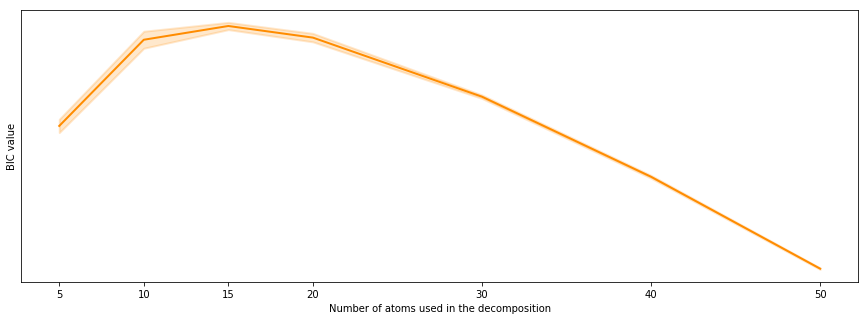
\includegraphics[scale=0.5]{parameterresearch.png}
\caption{Curve of the \texttt{scoring\_function} values (refined BIC) w.r.t. the number of atoms used for the decomposition. To an higher value corresponds a better model for the dataset. In this case the best model is the one with 15 atoms in the dictionary.}
\label{bic}
\end{figure}
%
%
%
%
%
\section{Appendix: interchangeability of the penalties} \label{penalty change}
With DALILA trying different penalties on the same dataset requires only few lines of code. 

For example suppose we have the right number of atoms (with the dataset we use is 7) in which to decompose the dataset and that, some oracle, told us the perfect regularisation parameters for each penalty on that dataset. Then we may want to try different sparsifications on the coefficients to see which one better approximates the original signal. We tried \texttt{L1Penalty}, \texttt{L0Penalty} and \texttt{ElasticNetPenalty}.

\begin{lstlisting}[language=Python]
import numpy as np

from dalila.dictionary_learning import DictionaryLearning
from dalila.dataset_generator import synthetic_data_non_negative
from dalila.penalty import L1Penalty, L0Penalty, ElasticNetPenalty

X, D, C = synthetic_data_non_negative()

estimator = DictionaryLearning(k=7, coeff_penalty=L1Penalty(0.01), non_negativity="both")
estimator.fit(X)
C_l1, D_l1 = estimator.decomposition()
error_l1 = estimator.reconstruction_error()

estimator = DictionaryLearning(k=7, coeff_penalty=L0Penalty(3), non_negativity="both")
estimator.fit(X)
C_l0, D_l0 = estimator.decomposition()
error_l0 = estimator.reconstruction_error()

estimator = DictionaryLearning(k=7, coeff_penalty=ElasticNetPenalty(0.01, 0.1, 0.7), non_negativity="both")
estimator.fit(X)
C_en, D_en = estimator.decomposition()
error_en = estimator.reconstruction_error()
\end{lstlisting}
After the execution of this piece of code the comparison between the results is straight-forward and you can notice that the effort is minimal. 

\section{Appendix: addition of a new penalty} \label{new penalty}
DALILA allows to easily introduce new customised penalties for the optimisation of dictionary learning or representation learning. We want to underline that, even if the implementation steps are easy, the function that computes the proximal mapping has to be correct and no theoretical inconsistencies should be present. The behaviour is otherwise unpredictable.  \\


The first step is the import of the super-class Penalty that our new penalty has to extend. We also import other things that we need later.
\begin{lstlisting}[language=Python]
from dalila.representation_learning import RepresentationLearning
from dalila.penalty import Penalty
import numpy as np
\end{lstlisting}
The implementation of the new class, besides the construction, has to expose the method \texttt{apply\_prox\_operator} that is the one called during the minimisation. In this method the prox operator is implemented. 
\begin{lstlisting}[language=Python]
class NewPenalty(Penalty):
    
    def __init__(self, regularization_parameter):
        self.regularization_parameter = regularization_parameter
	
	  # x is the matrix on which apply the prox
	  # gamma is the gradient descent step
    def apply_prox_operator(self, x, gamma): 
        # if you are declaring a real penalty
        # change the implementation and 
        # transform x according to your penalty
        return x

\end{lstlisting}
Once we have declared the penalty, in this case a penalty that does nothing, we put it into the representation learning procedure. 
\begin{lstlisting}[language=Python]
fake_data = np.random.rand(50,50)
fake_dictionary = np.random.rand(5, 50)
estimator = RepresentationLearning(fake_dictionary, penalty=NewPenalty(5))
estimator.fit(fake_data)
\end{lstlisting}\vspace{0.2cm}
It is also possible to use the parameter research procedures with the new penalty provided that we also overwrite the method \texttt{make\_grid} since the searching function assumes it exists. We here show a basic example of how it can be implemented, one may want to vary the interval or the sampling procedure. 
\begin{lstlisting}[language=Python]
class NewPenalty(Penalty):
   
	  # ..as above..
        
    def make_grid(self, low=0.001, high=1, number=10):
		# possible regularization parameters to analyse        
        values = np.linspace(low, high, number)
        l = []
        # the list has to be composed of NewPenalty objects
        for (i, v) in enumerate(values):
            l.append(NewPenalty(v))
        return l
\end{lstlisting}
Again we show that it is usable right away without further code.
\begin{lstlisting}[language=Python]
from dalila.parameters_research import tune_parameters_RL
estimator = RepresentationLearning(fake_dictionary, penalty=NewPenalty(5))
gscv = tune_parameters_RL(fake_data, estimator, coeff_penalty_range=(0.1, 1, 3))
\end{lstlisting}
